\documentclass[12pt]{article}
\usepackage[margin=1in]{geometry}
\usepackage{setspace}
\onehalfspacing

% Start of preamble
%==========================================================================================%
% Required to support mathematical unicode
\usepackage[warnunknown, fasterrors, mathletters]{ucs}
\usepackage[utf8x]{inputenc}

\usepackage[dvipsnames,table,xcdraw]{xcolor}
\usepackage{hyperref} 
\hypersetup{
colorlinks=true,
linkcolor=blue,
filecolor=magenta,
urlcolor=cyan,
pdfpagemode=FullScreen
}

% Standard mathematical typesetting packages
\usepackage{amsmath,amssymb,amscd,amsthm,amsxtra, pxfonts}
\usepackage{mathtools,mathrsfs,dsfont,xparse}

% Symbol and utility packages
\usepackage{cancel, textcomp}
\usepackage[mathscr]{euscript}
\usepackage[nointegrals]{wasysym}
\usepackage{apacite}

% Extras
\usepackage{physics}  
\usepackage{tikz-cd} 
\usepackage{microtype}
\usepackage{enumitem}
\usepackage{titling}
\usepackage{graphicx}

% Fancy theorems due to @intuitively on discord
\usepackage{mdframed}
\newmdtheoremenv[
backgroundcolor=NavyBlue!30,
linewidth=2pt,
linecolor=NavyBlue,
topline=false,
bottomline=false,
rightline=false,
innertopmargin=10pt,
innerbottommargin=10pt,
innerrightmargin=10pt,
innerleftmargin=10pt,
skipabove=\baselineskip,
skipbelow=\baselineskip
]{mytheorem}{Theorem}

\newenvironment{theorem}{\begin{mytheorem}}{\end{mytheorem}}

\newtheorem{corollary}{Corollary}
\newtheorem{lemma}{Lemma}

\newtheoremstyle{definitionstyle}
{\topsep}%
{\topsep}%
{}%
{}%
{\bfseries}%
{.}%
{.5em}%
{}%
\theoremstyle{definitionstyle}
\newmdtheoremenv[
backgroundcolor=Violet!30,
linewidth=2pt,
linecolor=Violet,
topline=false,
bottomline=false,
rightline=false,
innertopmargin=10pt,
innerbottommargin=10pt,
innerrightmargin=10pt,
innerleftmargin=10pt,
skipabove=\baselineskip,
skipbelow=\baselineskip,
]{mydef}{Definition}
\newenvironment{definition}{\begin{mydef}}{\end{mydef}}

\newtheorem*{remark}{Remark}

\newtheorem*{example}{Example}

% Common shortcuts
\def\mbb#1{\mathbb{#1}}
\def\mfk#1{\mathfrak{#1}}

\def\bN{\mbb{N}}
\def \C{\mbb{C}}
\def \R{\mbb{R}}
\def\bQ{\mbb{Q}}
\def\bZ{\mbb{Z}}
\def \cph{\varphi}
\renewcommand{\th}{\theta}
\def \ve{\varepsilon}
\newcommand{\mg}[1]{\| #1 \|}

% Often helpful macros
\newcommand{\floor}[1]{\left\lfloor#1\right\rfloor}
\newcommand{\ceil}[1]{\left\lceil#1\right\rceil}
\renewcommand{\qed}{\hfill\qedsymbol}
\renewcommand{\P}{\mathbb P\qty}
\newcommand{\E}{\mathbb{E}\qty}
\newcommand{\Cov}{\mathrm{Cov}\qty}
\newcommand{\Var}{\mathrm{Var}\qty}

% Sets
\usepackage{braket}

\graphicspath{{/}}
\usepackage{float}

\newcommand{\SET}[1]{\Set{\mskip-\medmuskip #1 \mskip-\medmuskip}}

% End of preamble
%==========================================================================================%

% Start of commands specific to this file
%==========================================================================================%

\usepackage{algorithm}
\usepackage{algpseudocode}
\newcommand{\OPT}{\mathrm{OPT}}

%==========================================================================================%
% End of commands specific to this file

\title{CSE 421 HW6}
\date{\today}
\author{Rohan Mukherjee}

\begin{document}
    \maketitle
    \subsection*{Problem 1.}
    Our algorithm is as follows:
    \begin{algorithm}
        \caption{2-Approximation to Bounded Knapsack}
        \begin{algorithmic}
            \Procedure{Bk}{$w, v, W$}
                \State Sort $w$ and $v$ in decreasing order of $\frac{v_i}{w_i}$
                \State $S \gets []$
                \State $w' \gets 0$
                \For{$i = 1$ to $n$}
                    \If{$w' < W$}
                        \If{$w' + w_i \leq W$}
                            \State $S.\mathrm{append}(i)$
                            \State $w' \gets w' + w_i$
                        \Else
                            \State $S.\mathrm{append}(\frac{W - w'}{w_i} i)$
                        \EndIf
                    \EndIf
                \EndFor
                \If{$S[-1]$ is a fraction}
                    \If{$v_{S[-1]} \geq \frac 12 \displaystyle \sum_{i \in S} v_i$}
                        \State \Return \text{non fractional variant of $S[-1]$}
                    \Else 
                        \State \Return $S.\mathrm{remove}(S[-1])$
                    \EndIf
                \EndIf
            \EndProcedure
        \end{algorithmic}
    \end{algorithm}
    The above algoritm works because the value returned by the ordinary fractional knapsack is an upper bound for the value of OPT in our case. Then we see if the fractional term we add is at least 1/2 of the total value in the knapsack, and output that one if that is the case. Otherwise, we throw away the fractional term and output the rest. This is a 2-approximation because either the value of the fractional term in the knapsack is at least half the value of the total knapsack or not, and we output the one with the higher value which is guarenteed to be at least half of the fractional output, which is at least half of the optimal value by the hint. Our algorithm clearly runs in $O(n \log n)$ time since we have to sort and the rest of the for loops take $O(n)$ time.

    \subsection*{Problem 2.}
    Our algorithm is as follows:
    \begin{algorithm}
        \caption{Biggest Value Rectangle}
        \begin{algorithmic}
            \Procedure{Bvr}{A}
            \State $O \gets n \times n \times n$ tensor of $0$
            \For{$1 \leq j \leq n$}
                \For{$1 \leq w \leq j$}
                    \State $O[1, j, w] \gets \max\SET{0, \displaystyle \sum_{k=j-w+1}^j A[1,k]}$
                \EndFor
            \EndFor
            \For{$2 \leq i \leq n$}
                \For{$1 \leq j \leq n$}
                    \State $r \gets 0$
                    \For{$1 \leq w \leq j$}
                        \State $r \gets r + A[i, j-w+1]$
                        \State $O[i,j,w] \gets \max \SET{r + O[i-1, j, w], 0}$
                    \EndFor
                \EndFor
            \EndFor
            \State \Return $\displaystyle \max_{i, j, w} O[i,j,w]$
            \EndProcedure
        \end{algorithmic}
    \end{algorithm}

    Let $\OPT(i,j,w)$ be the optimal rectangle of width $w \leq j$, where the height can possibly be 0 (resulting in the empty rectangle), with $(i,j)$ as the bottom right corner. We proceed by induction on $i$. In the case where $i = 0$, we know have also specified the height to be either 0 or 1, since the bottom right corner of the rectangle has index 1. It then follows immediately that for each $j$ and $1 \leq w \leq j$, we the optimal and only rectangle of width $w$ with height $\leq 1$ is just going to be
    \begin{align*}
        \max \SET{0, \sum_{k=j-w+1}^j A[1, k]}
    \end{align*}
    where the first entry in the max is taken if the only rectangle with width $w$ and height $1$ with bottom right corner $(1, j)$ has negative weight. Now, notice that the optimal rectangle with width $w$ with $(i,j)$ as the bottom right corner can be found by doing the following. Inductively, $\OPT(i-1, j, :)$ holds the right value, so we know that the optimal rectangle of width $w$, and bottom right corner $(i, j)$ is simply going to be the optimal rectangle of width $w$ and bottom right corner $(i-1, j)$ plus the final row we have added on the bottom, where the optimal rectangle with bottom right corner of $(i-1, j)$ of width $w$ can possibly be empty, or 0 if this sum happens to be negative. Thus we get the following formula, for $1 \leq w \leq j$,
    \begin{align*}
        \OPT(i,j,w) = \max \SET{\OPT(i-1,j,w) + \sum_{k=j-w+1}^j A[i, k], 0}.
    \end{align*}
    The last step is to take the maximum over all valid $i,j,w$, and since the optimal rectangle will have a bottom right corner and a width, this algorithm is correct.

    We see that the first nested for loop takes $O(n^3)$ time, because the sum can certainly be found in $O(n)$ time. The second for loop has two inner steps that both take $O(1)$ time, where we save the value of the row sum $\sum_{k=j-w+1}^j A[i,k]$ in $r$ and can update it to find the correct row sum for the next $w$ in $O(1)$ time. In this way the triple nested for loop takes only $O(n^3)$ time. The last max is over $\leq n^3$ elements and hence our algorithm runs in $O(n^3)$ time.

    \subsection*{Problem 3.}
    First assign $T$ a root $v$, and then run the following algorithm, and then extract the first item from the returned tuple:

    \newpage


    \begin{algorithm}
        \caption{Number of Connected Subsets}
        \begin{algorithmic}
            \Procedure{Ncs}{$T, k$}
            \If{$T$ is a single vertex}
                \State \Return $(1, [1] + [0] * k)$
            \EndIf
            \State $v \gets \text{root of } T$
            \State $n \gets \text{number of neighbors of } v$
            \State $A \gets [0] * k$
            \State $A[0] \gets 1$
            \If{$\deg v = 1$}
                \State $T, B \gets \Call{Ncs}{T-v, k}$
                \For{$i = 1$ to $k$}
                    \State $A[i] \gets B[i-1]$
                \EndFor
                \State \Return $(T+A[k], A)$
            \EndIf
            \EndProcedure
            \If{$\deg v = 2$}
                \State $C_1, C_2 \gets \text{ connected components of } T-v \text{ with roots being $v$'s neighbors}$
                \State $T_1, B \gets \Call{Ncs}{C_1, k}$
                \State $T_2, C \gets \Call{Ncs}{C_2, k}$
                \For{$\ell = 1$ to $k$}
                    \For{$i + j = \ell-1$}
                        \State $A[\ell] \gets B[i]C[j]$
                    \EndFor
                \EndFor
                \State \Return $(T_1+T_2+A[k], A)$
            \EndIf
            \If{$\deg v = 3$}
            \State $C_1, C_2, C_3 \gets \text{ connected components of } T-v \text{ with roots being $v$'s neighbors}$
            \State $T_1, B \gets \Call{Ncs}{C_1, k}$
            \State $T_2, C \gets \Call{Ncs}{C_2, k}$
            \State $T_3, D \gets \Call{Ncs}{C_3, k}$
                \For{$\ell = 1$ to $k$}
                    \For{$i + j + m = \ell-1$}
                        
                        \State $A[\ell] \gets B[i]C[j]D[m]$
                    \EndFor
                \EndFor
                \State \Return $(T_1+T_2+T_3+A[k], A)$
            \EndIf
        \end{algorithmic}
    \end{algorithm}


    The below (I do not know how to typset it above) algorithm works by partioning into cases. We first root the tree $T$ with $v$. Suppose that $\deg v = 3$. Then removing $v$ from $T$ will yield 3 connected components $C_1, C_2, C_3$ with roots being the neighbors $w_1, w_2, w_3$ of $v$. To find the number of connected subsets of $T$ with $k$ elements, we sum over $i + j + m = \ell-1$ by putting together a path of length $i$ from the first connected component, $j$ from the second and $m$ from the third, which can be done in $B[i]C[j]D[m]$ ways if we store the number of connected subsets with $w_i$ as a root in $B, C, D$ respectively. The last thing is to decree that the number of connected subsets with $0$ elements to be 0 so that the multiplication works out. Finally we can keep a running total of the number of $k$ sized connected subset by noticing that the number of $k$ sized connected subset of the entire graph is either going to be a $k$ sized connected subset of one of the connected components, or is going to use $v$ as a bridge between two or more connected components, which we have already calculated and stored in $A$. The time complexity is complicated once again, but we get something of the following type:
    \begin{align*}
        T(n) = \sum_{(v,w_i) \in E} T(|C_i|) + O(k \cdot n^3)
    \end{align*} 
    This because the third for loop is easily seen to be the most expensive part of the algorithm, and there are ${n + 3 - 1 \choose 3} = O(n^3)$ loop iterations (by stars and bars), all of which take $O(1)$ time, which is being run inside of a bigger for loop iterating over $\ell$ which runs through $k$. Then we call the algorithm recursively on the connected components who have total number of vertices summing to $n-1$. Thus our time complexity is as above. I have shown on a previous homework that $\sum_{(v,w_i) \in E} T(|C_i|) \leq T(n-1)$ because $T$ is growing at least polynomially, and hence we see that $T(n) \leq T(n-1) + O(n^3)$ in any case which shows that $T(n) = O(k \cdot n^4) \leq O(n^5)$ because $k \leq n$.

    \newpage
    \subsection*{Problem 4.}
    The residual graph I got is:

    \begin{figure}[H]
        \centering
        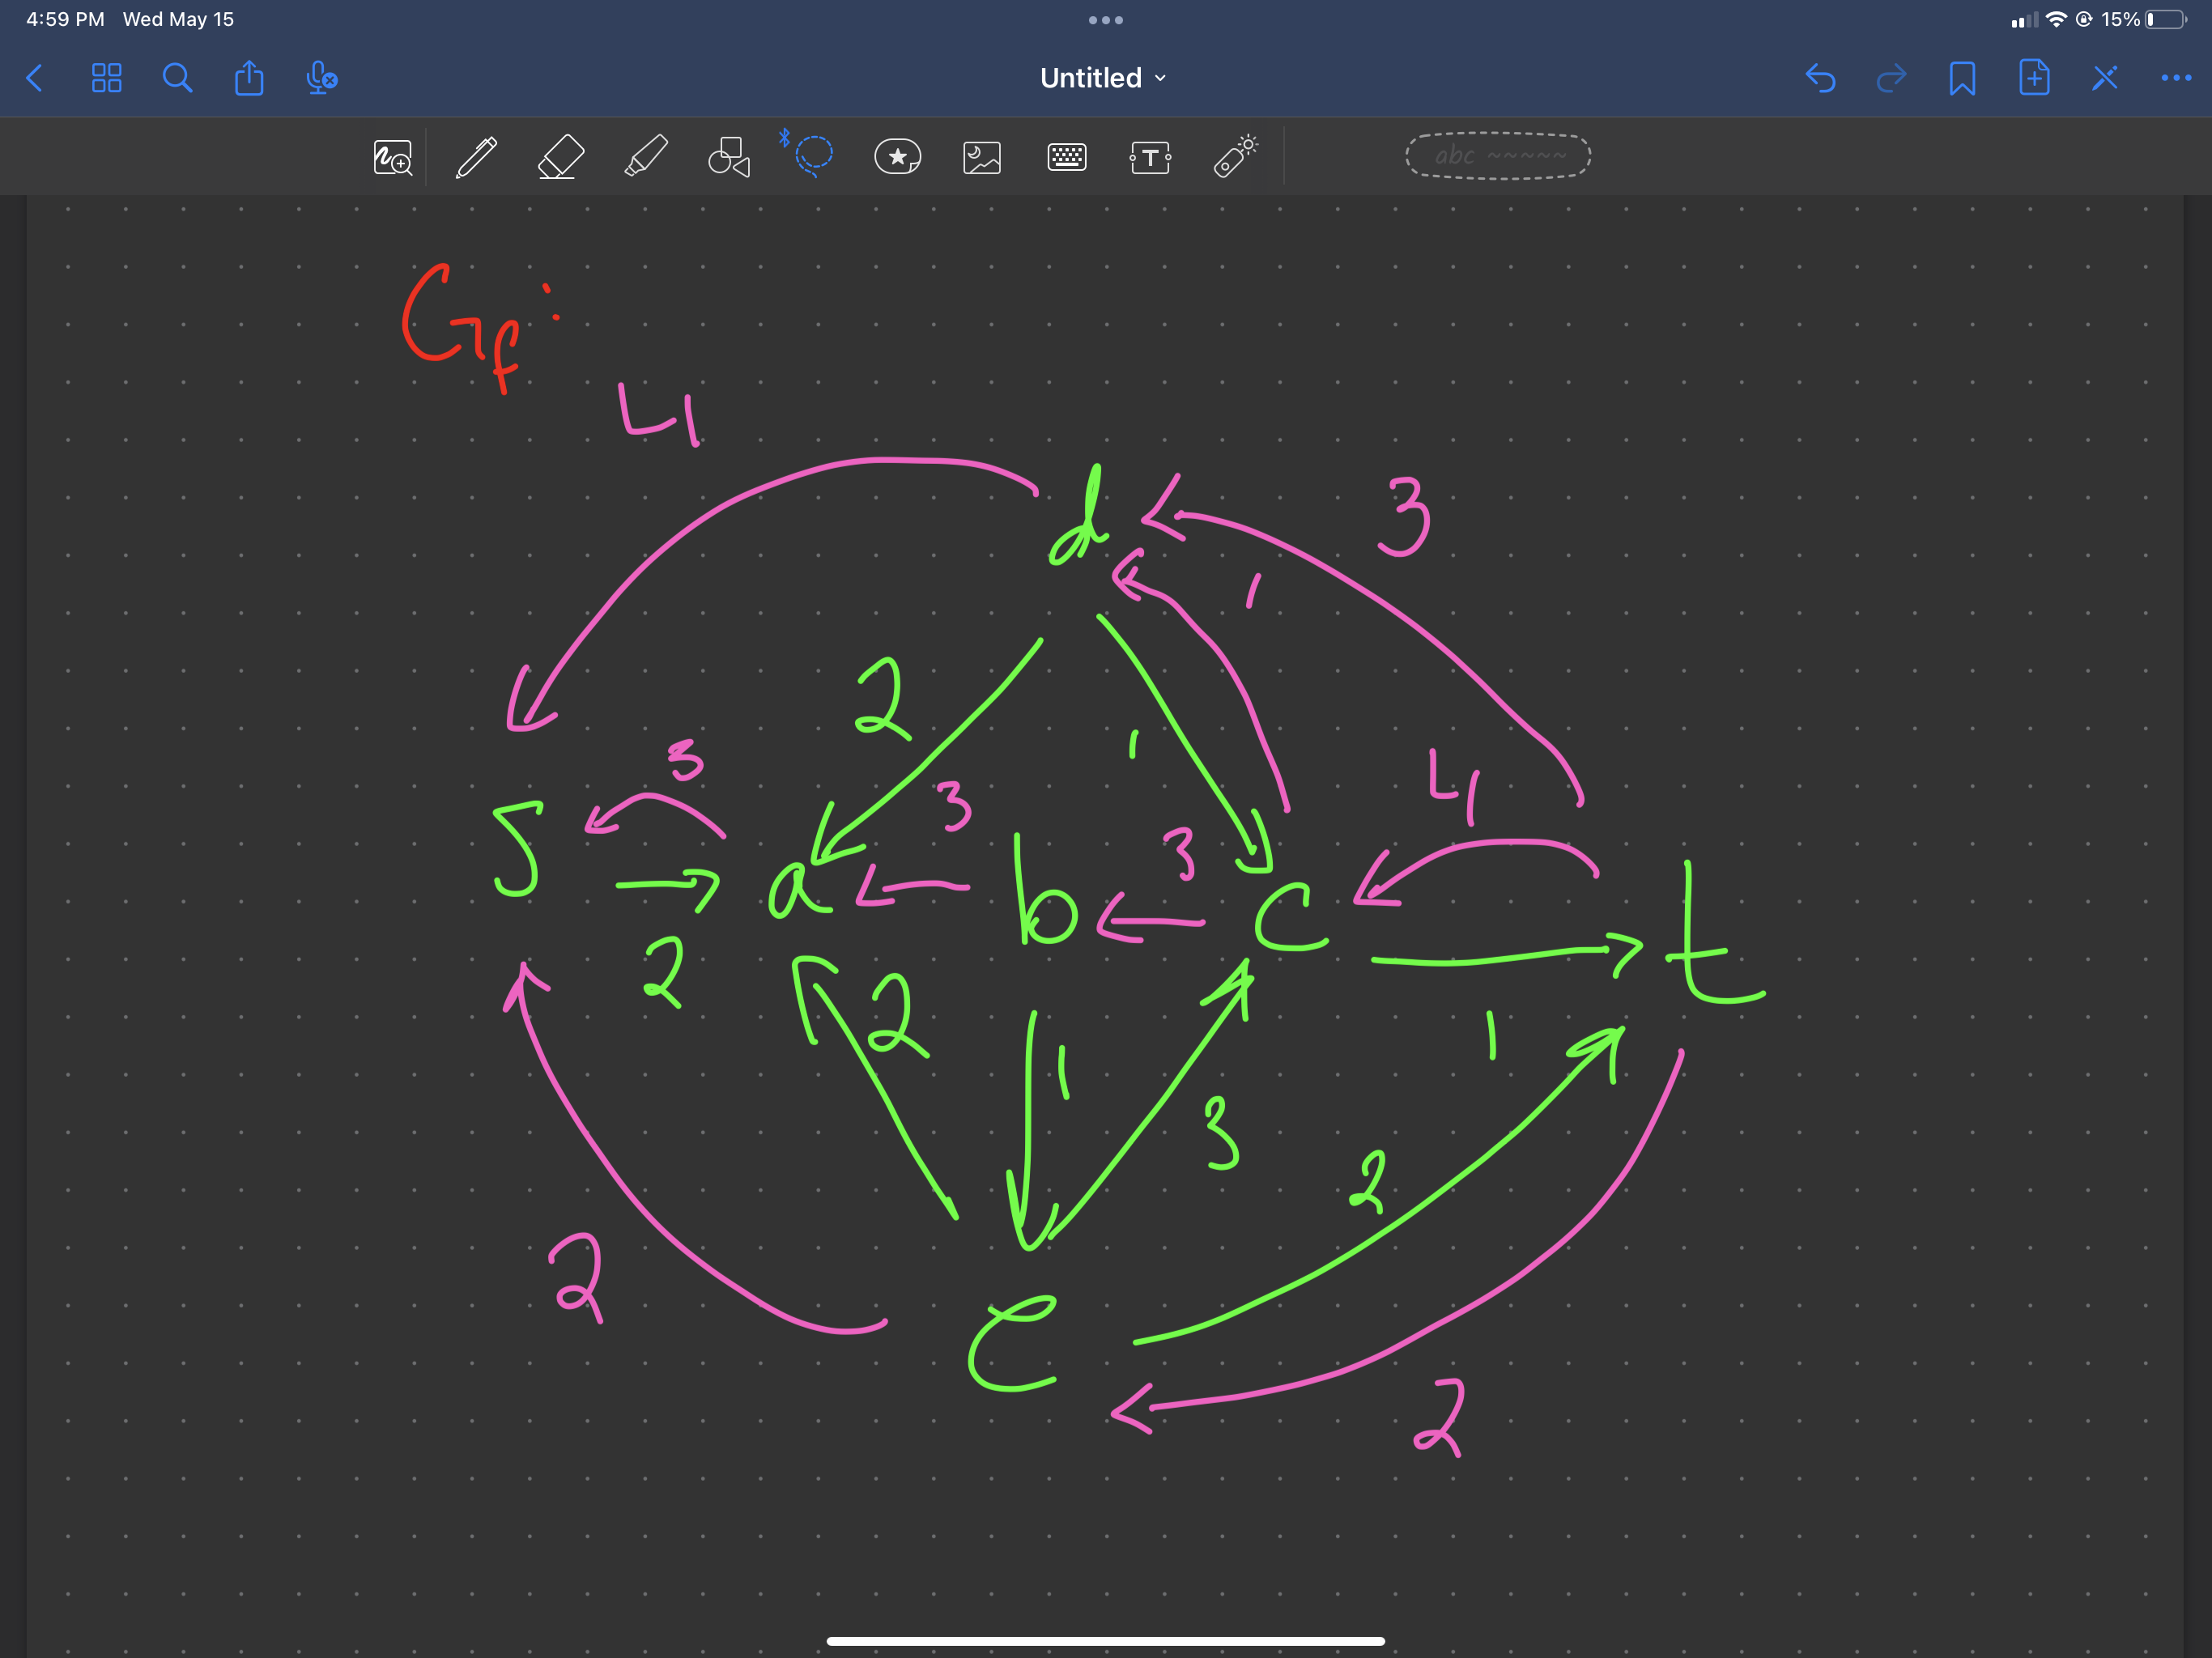
\includegraphics[width=0.7\textwidth]{residual.png}
    \end{figure}
    The flow and cut I got are:

    \begin{figure}[H]
        \centering
        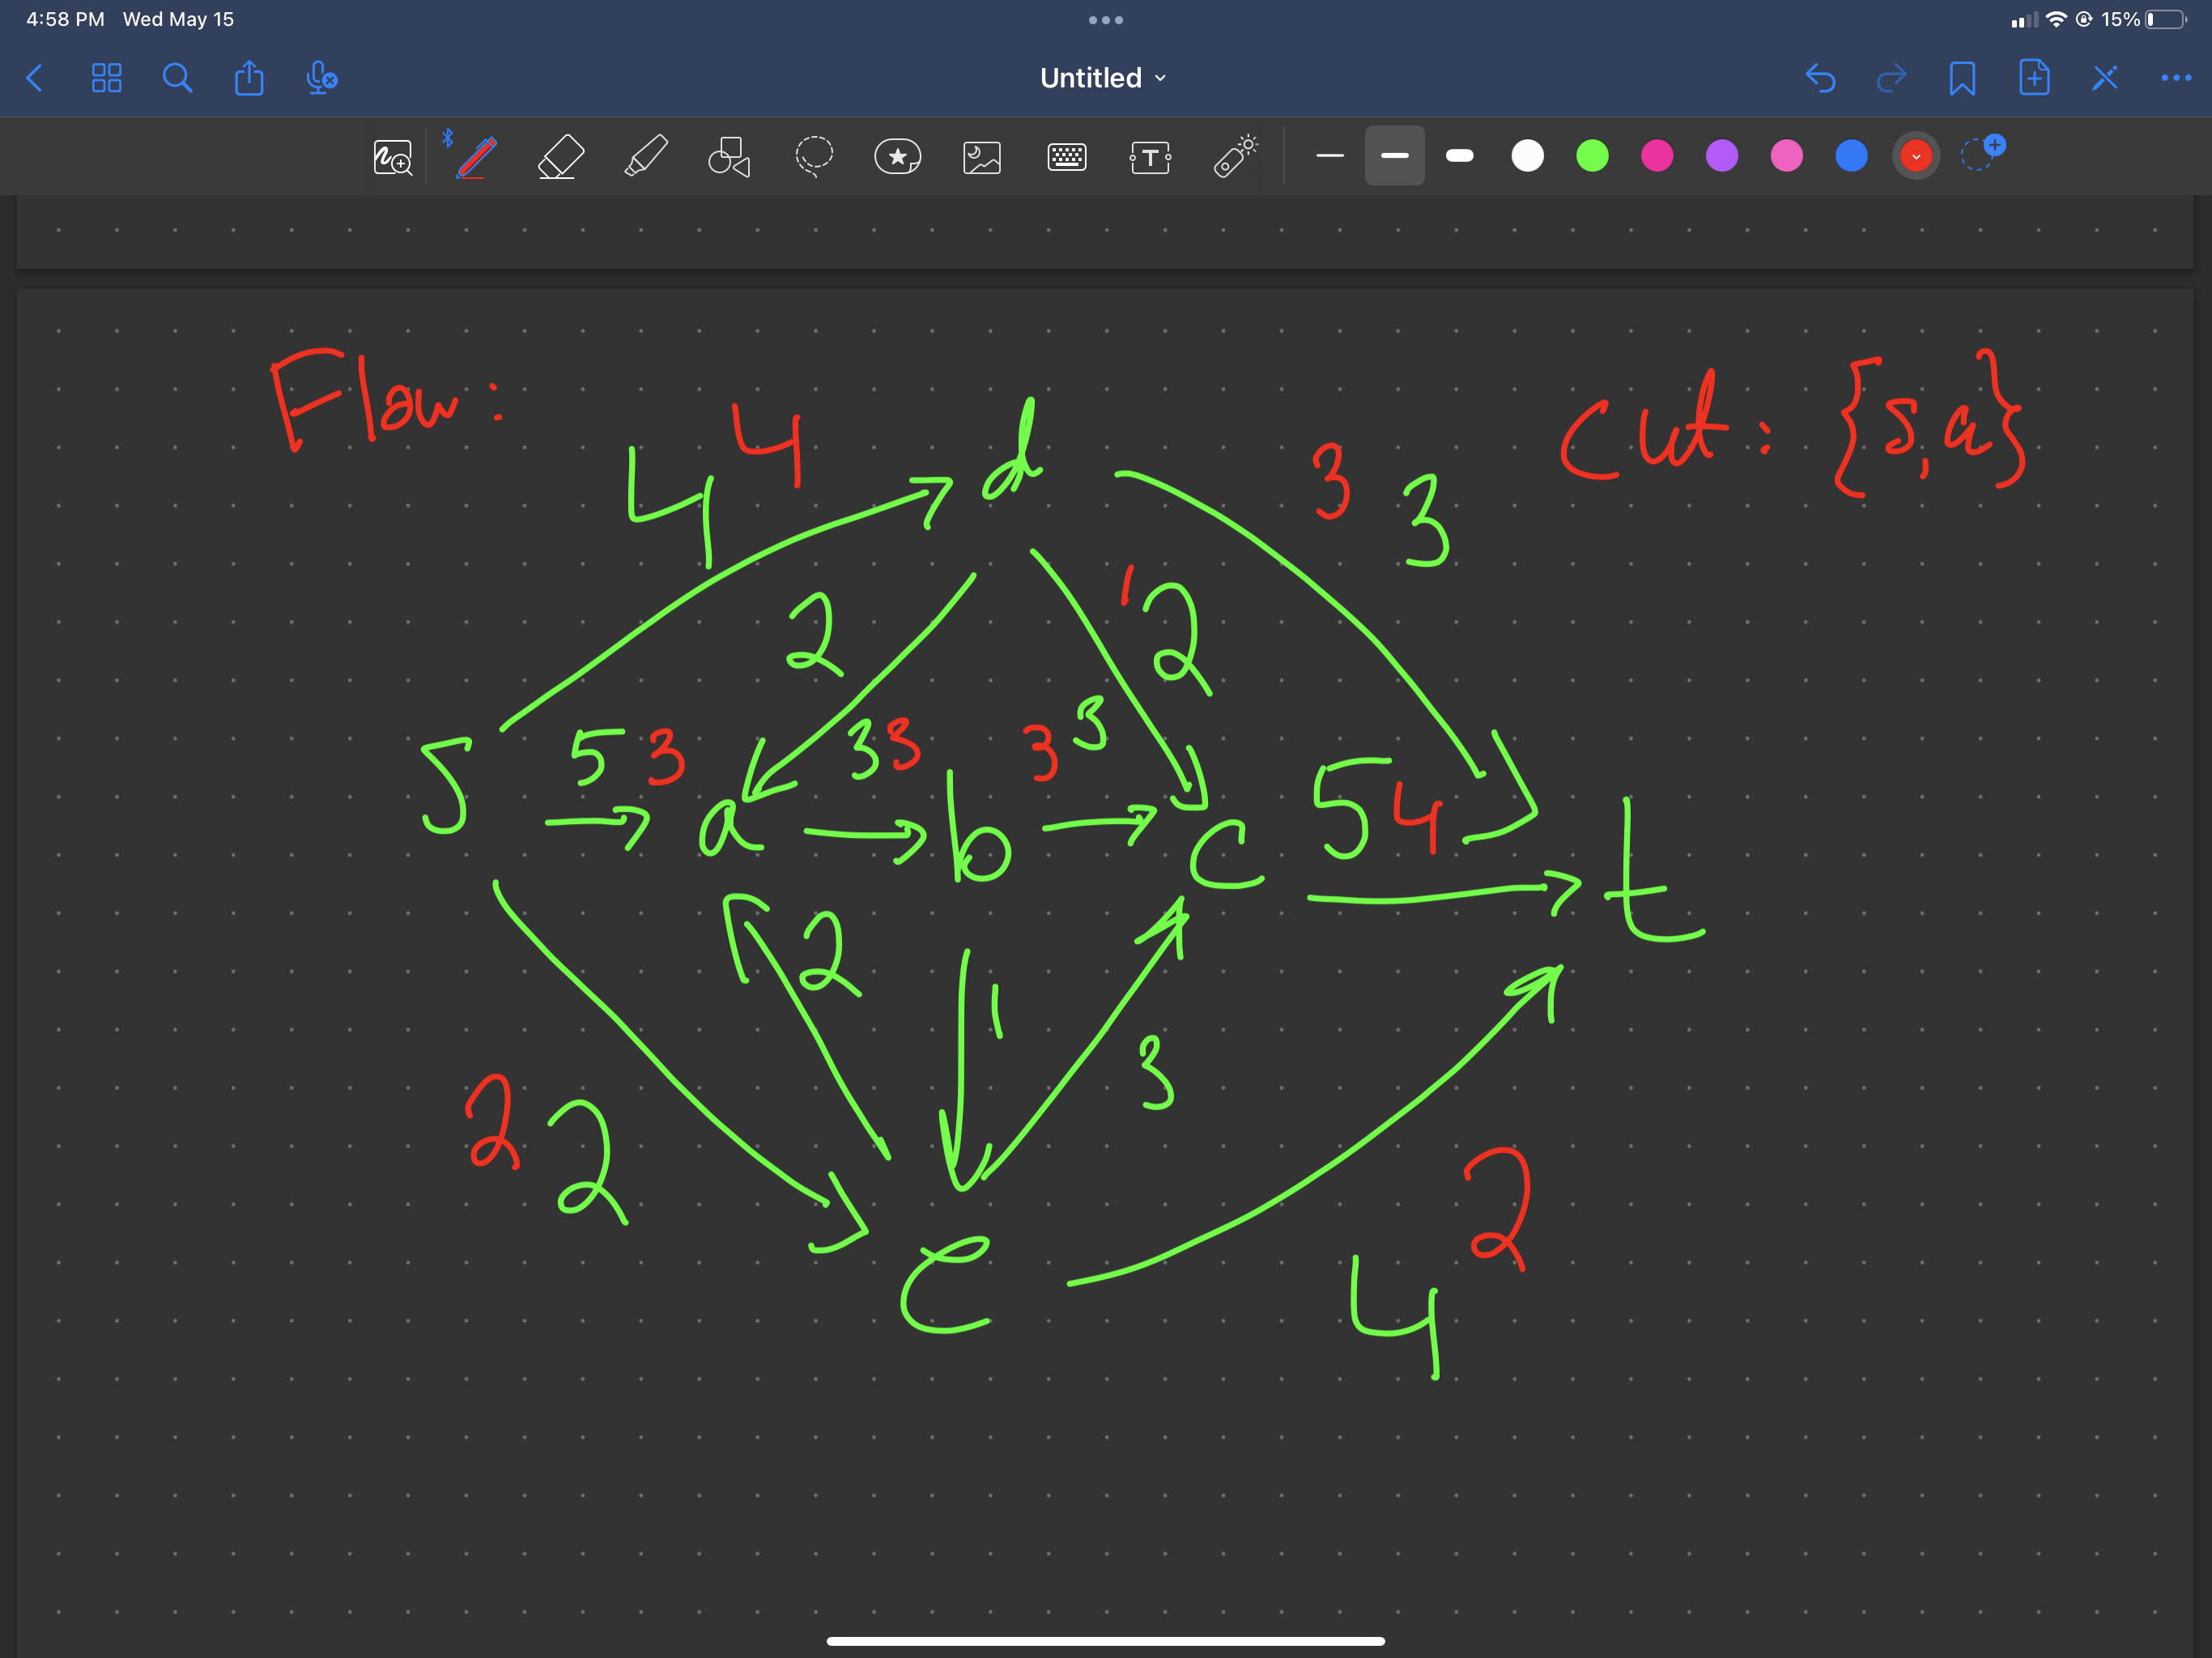
\includegraphics[width=0.7\textwidth]{flow_cut.png}
    \end{figure}
\end{document}